% How to make a flowchart using tikz package
% Made in 2018 by Luis Plata: https://github.com/LuisPlata94/LaTeX-Presentation

% Based on different guides:
% ShareLaTeX's beamer guide: https://es.sharelatex.com/learn/Beamer

\documentclass[12pt]{beamer}

% Changing the appearance
\setbeamertemplate{navigation symbols}{} % Hides the navigation bar
\setbeamertemplate{caption}[numbered] % Numerates the images
\usetheme{Madrid} % Theme 
\usecolortheme{default} % Colors http://deic.uab.es/~iblanes/beamer_gallery/index_by_theme.html
%\usefonttheme{structuresmallcapsserif} % Changes font
%\usepackage{bookman} % Changes font

% Loading tiks and defining diferent shapes
\usepackage{tikz}
\usetikzlibrary{shapes.geometric, arrows}
\tikzstyle{ss} = [rectangle, rounded corners, minimum width=0.5cm, minimum height=0.5cm,text centered, draw=black, fill=red!30]
\tikzstyle{inp} = [trapezium, trapezium left angle=70, trapezium right angle=110, minimum width=0.5cm, minimum height=0.5cm, text centered, draw=black, fill=blue!30]
\tikzstyle{pro} = [rectangle, minimum width=0.5cm, minimum height=0.5cm, text centered, draw=black, fill=orange!30]
\tikzstyle{dec} = [diamond, aspect=2, minimum width=0cm, minimum height=0cm, text centered, draw=black, fill=green!30]
\tikzstyle{con} = [circle, draw=white]
\tikzstyle{arrow} = [thick,->,>=stealth]

\begin{document}
	
\begin{frame}
\frametitle{A flowchart}
\begin{center}
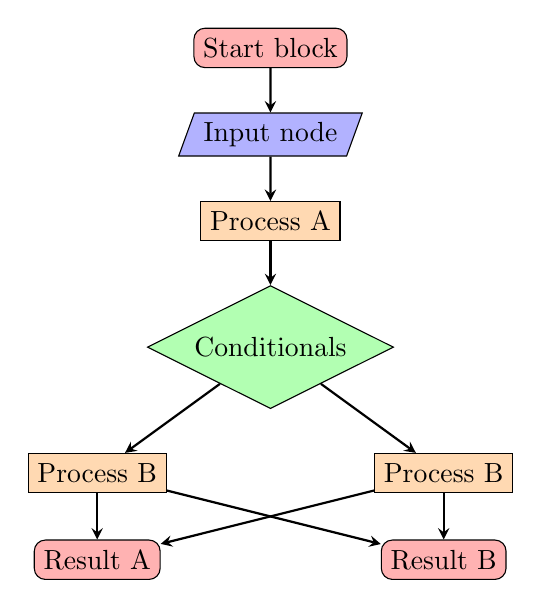
\begin{tikzpicture}[node distance=1.1cm]
% Drawing nodes
\node (start) [ss] {Start block};
\node (in1) [inp, below of=start] {Input node};
\node (pro1) [pro, below of=in1]  {Process A};
\node (dec1) [dec, below of=pro1, yshift=-0.5cm]  {Conditionals};
\node (pro2) [pro, below of=dec1, xshift=-2.2cm, yshift=-0.5cm]{Process B};
\node (pro3) [pro, below of=dec1, xshift=2.2cm, yshift=-0.5cm]{Process B};
\node (end1) [ss, below of=pro2] {Result A};
\node (end2) [ss, below of=pro3] {Result B};

% Drawing arrows
\draw [arrow] (start) -- (in1);
\draw [arrow] (in1) -- (pro1);
\draw [arrow] (pro1) -- (dec1);
\draw [arrow] (dec1) -- (pro2);
\draw [arrow] (dec1) -- (pro3);
\draw [arrow] (pro2) -- (end1);
\draw [arrow] (pro2) -- (end2);
\draw [arrow] (pro3) -- (end1);
\draw [arrow] (pro3) -- (end2);
\end{tikzpicture}
\end{center}
\end{frame}

\end{document}


